\chapter[Структура проекта. Основные типы]{\bfseries Структура проекта. Основные типы}
\section[Файлы проекта]{Файлы проекта}
Теперь давайте рассмотрим из чего состоит проект \Sys{Qt}. В общем, проект \Sys{Qt}
имеет такую структуру:

\begin{itemize}
\item \index{Файл!проекта}файл проекта --- описывает файлы,
которые входят в проект и содержит необходимые настройки;
\item файлы, входящие в проект (или другие подпроекты, если проект разбит на несколько частей).
\end{itemize}
Ключевую роль имеет файл проекта с расширением \index{Расширение файла!.pro}\Sys{.pro}.
Он содержит списки файлов: исходных кодов, файлов ресурсов, файлов локализации, форм, других файлов,
которые входят в проект, а также файлов подпроектов, если
проект состоит с нескольких частей. Этот файл также содержит некоторые настройки программы.

Теперь рассмотрим создание своего \index{Создание!проектного файла}проектного файла. Создадим новую папку, 
где будет размещаться проект (например: \Sys{custom\_project}). Создайте файл (это будет файл 
проекта) введите его имя с расширением \Sys{.pro} (например:
\Sys{custom\_project.pro}). Наш файл пока что пустой, но его уже можно открыть в \Sys{Qt Creator} 
(воспользуйтесь главным меню: \Sys{File->Open File or Project...}). 

Создать \index{Создание!пустого проекта}пустой проект можно с
помощью  мастера построения проектов. Для этого надо воспользоваться главным меню 
\Sys{File->New File or Project...} либо комбинацией клавиш \Sys{Ctrl+Shift+N}. В 
окне мастера нужно выбрать раздел \Sys{Other Project} (Другой проект) и тип 
проекта --- \Sys{Empty Qt Project}.

После того, как мы открыли проект, \Sys{Qt Creator} предлагает выбрать комплект
для его компиляции. В разделе \Sys{Projects} (Проекты) выберем
комплект по умолчанию и нажмём Configure
Project. В дереве проекта выберем  и откроем файл проекта. Теперь настало время
исследовать синтаксис проектных файлов~\Sys{Qt}.

Проектный файл обычно содержит несколько настроек в виде специальных переменных, каждая из которых играет
свою особую роль. Среди большого количества настроек, которые задают в \Sys{.pro}-файле:

\begin{itemize}
\item тип проекта (приложение, динамическая или статическая библиотека, проект, который состоит из
подпроектов);
\item общие настройки проекта;
\item настройки компиляции;
\item путь, где будет размещён исполняемый файл, библиотека или бинарный
файл во время процесса компиляции;
\item пути к файлам, библиотекам и другим
частям проекта необходимым для компиляции;
\item файлы, входящие в проект;
\item дополнительные действия, которые будут выполняться в процессе компиляции проекта.
\end{itemize}

Откройте проектный файл и добавьте к нему содержимое. Обратите внимание: символ \#
можно использовать для обозначения комментариев.
\begin{lstlisting}
# `Указываем тип проекта`
TEMPLATE = app # app - Application, `прикладная программа`
# `Используемые модули` Qt 
QT -= gui # `Удаляем из списка модуль` gui
# `это означает отказ от использования графического интрефейса,`
# `то есть --- консольную программу`
CONFIG += console # `Конфигурируем создание консольного проекта`
# `(нужно только для консольных проектов в Windows, в Linux и Mac OS X не выполняет никаких действий)`
CONFIG -= app_bundle # `Предотвращает создание Application bundle в` Mac OS X
# `(нужно только для консольных проектов в Mac OS X)`
TARGET = custom_project # `Название исполняемого файла`
\end{lstlisting}

\index{Создание!файла исходных текстов}Теперь нам осталось добавить в проект
файл с текстом программы. Для этого мы снова можем воспользоваться мастером. 
В категории \Sys{Files and Classes (Файлы и классы)} выберем раздел \Sys{C++} и выберем тип файла
<<\Sys{C++ Source File}>> (Файл исходных текстов \Sys{C++}).
Поскольку это будет главный файл программы, то дадим ему привычное для
этого случая название: \Sys{main.cpp}. Текст программы является обычным:
\begin{lstlisting}
int main(int lArgc, char *lArgv[])
{
  return 0;
}
\end{lstlisting}

После создания \Sys{main.cpp}, вновь откроем файл проекта и обратим внимание на несколько дополнительных строк:
\begin{lstlisting}
SOURCES += \
    main.cpp
\end{lstlisting}

Переменная \index{Переменные qmake!SOURCES}\Sys{SOURCES} хранит список \Sys{.cpp}
файлов. В табл.~\ref{ch12:refTable0} мы предоставляем список переменных, которые часто участвуют в
описании проекта:

{\noindent\small\tabcolsep=0.5em
\begin{longtable}{|p{0.17\textwidth}|p{0.43\textwidth}|p{0.32\textwidth}|}
\caption{Некоторые важные переменные для описания настроек проекта} \label{ch12:refTable0}\\
\hline
\Emph{Переменная}&\Emph{Описание}&\Emph{Пример}\\
\hline \hline
\endfirsthead
\multicolumn{3}{c}%
{{\tablename\ \thetable{} --- продолжение}} \\
\hline
\Emph{Переменная}&\Emph{Описание}&\Emph{Пример}\\
\hline \hline
\endhead
\index{Переменные qmake!CONFIG}\Sys{CONFIG} &Разнообразные настройки конфигурации проекта (например: режим отладки, вывод предупреждений, компиляция динамической библиотеки и~т.п.). &
\lstinline!CONFIG += dll plugin \!\linebreak
\lstinline!    warn_on release!\\\hline
\index{Переменные qmake!DEFINES}\Sys{DEFINES} &Макроопределения в проекте. Работает так же, как директива препроцессора \#define. &
\lstinline!DEFINES += DEBUG_OUTPUT \!\linebreak
\lstinline!    CUSTOM_DEFINE!\\\hline
\index{Переменные qmake!DESTDIR}\Sys{DESTDIR} &Путь к папке, где будет создан исполняемый файл. 
&\lstinline!DESTDIR = ./bin!\\\hline
\index{Переменные qmake!INCLUDEPATH}\Sys{INCLUDEPATH} &Путь к папкам с заголовочными файлами. &
\lstinline!INCLUDEPATH += ./includes \!\linebreak
\lstinline!    ./my_header_files!\\\hline
\index{Переменные qmake!FORMS}\Sys{FORMS} &Файлы форм \Sys{Qt} Designer. &
\lstinline!FORMS += mainwindow.ui!\\\hline
\index{Переменные qmake!HEADERS}\Sys{HEADERS} &Заголовочные файлы программы~\Sys{*.h}.&
\lstinline!HEADERS += mainwindow.h!\\\hline
\index{Переменные qmake!LIBS}\Sys{LIBS} &Пути к динамическим библиотекам и библиотеки, которые используются в программе. &
\lstinline!LIBS += -L./libs \!\linebreak
\lstinline!    -L./my_libs \!\linebreak
\lstinline!    -lmycustomlib!\\\hline
\index{Переменные qmake!QT}\Sys{QT} &Модули \Sys{Qt}, которые используются в программе. &
\lstinline!QT += core gui widgets \!\linebreak
\lstinline!    network sql xml!\\\hline
\index{Переменные qmake!RESOURCES}\Sys{RESOURCES} &Файл ресурсов. &
\lstinline!RESOURCES = resources.qrc!\\\hline
\index{Переменные qmake!SOURCES}\Sys{SOURCES} &Исходные тексты программы \Sys{*.cpp}. &
\lstinline!SOURCES += main.cpp \!\linebreak
\lstinline!    mainwindow.cpp!\\\hline
\index{Переменные qmake!TARGET}\Sys{TARGET} &Название исполняемого файла или динамической библиотеки. &
\lstinline!TARGET = MyFirstProject!\\\hline
\index{Переменные qmake!TEMPLATE}\Sys{TEMPLATE} & Тип проекта (приложение, библиотека, составленный из подпроектов ...) &
\lstinline!TEMPLATE = lib!\\\hline
\end{longtable}
}

\section[Компиляция проекта]{Компиляция проекта}
\index{Компиляция проекта}Компиляция проекта проходит в два этапа. Сначала
выполняется предварительная обработка проекта с помощью программы \index{Инструменты Qt!qmake}\Sys{qmake}.
Этот инструмент \Sys{Qt} несёт ответственность за весь процесс компиляции проекта. Он читает содержание
проектного файла и генерирует необходимые промежуточные файлы (дополнительные файлы с исходным кодом и
\index{Файл!make-файл}\Sys{make}-файлы для компиляции). Это необходимо для того,
чтобы превратить все особые расширения \Sys{Qt}, которые были использованы в программе, 
в код на языке \Sys{C++} и использовать
дополнительные настройки для проекта, описанные в
\Sys{pro}-файле. После этого проект готов к обработке компилятором. Вторым этапом
является непосредственно процесс компиляции. Все эти действия выполняются автоматически в среде \Sys{Qt Creator}.

\begin{figure}[htb]
\begin{center}
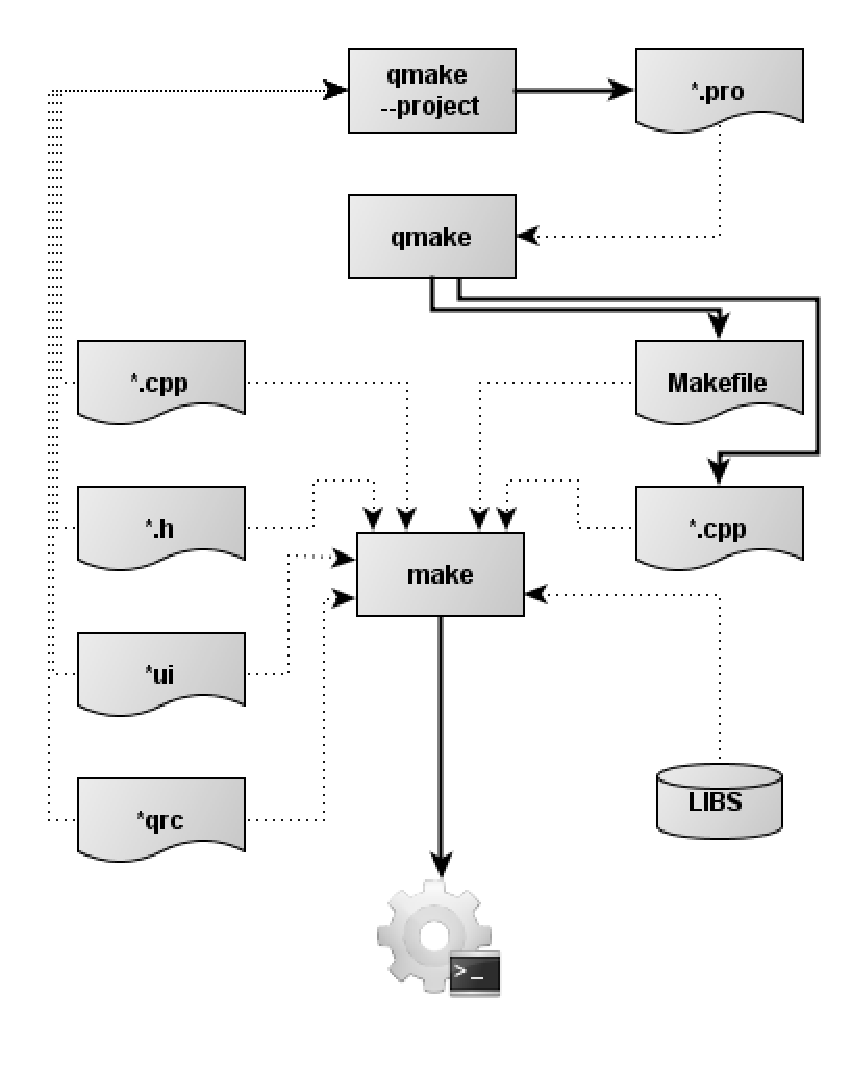
\includegraphics[width=0.7\textwidth]{img/ris_12_1}
\caption{Процесс компиляции проекта}
\label{ch12:refDrawing0}
\end{center}
\end{figure}

После успешной компиляции мы получаем исполняемый файл программы. Откройте папку проекта. Она будет
содержать исполняемый файл и все промежуточные файлы, сгенерированные в процессе.

Таким образом, процессом построения проекта руководит \Sys{.pro}-файл. При наличии исходных текстов программы и
при отсутствии. \Sys{pro}-файла, его можно сгенерировать. Для этого из командной строки
необходимо перейти в папку, которая содержит исходные тексты программы и вызвать \Sys{qmake}
с параметром -{-}\Sys{project}. Этим приёмом удобно
воспользоваться, чтобы сгенерировать файл проекта и использовать оболочку \Sys{QtCreator}
для работы над программой (даже для обычных программ на \Sys{C++} без \Sys{Qt}).

Раздел <<\Sys{Projects}>> (Проекты) содержит набор
необходимых настроек для процесса компиляции и для настройки среды запуска проекта. Одной
из таких настроек есть опция \index{Настройка!Shadow Build}\Sys{Shadow Build}, которая 
позволяет включить режим при котором для промежуточных файлов,
\Sys{make}-файлов и продуктов компиляции создаётся отдельная папка вне папки с исходным кодом проекта
(настройки размещения для неё --- в поле \Sys{Build directory}). Это позволяет построить и
хранить одновременно несколько вариантов построенного проекта для различных инструментариев. Также это сохраняет папку
с исходным кодом от засорения файлами, созданными в процессе построения проекта. При выключенном \Sys{Shadow
build} промежуточные файлы и папка с построенной программой сохраняются в папке, которая содержит файл
проекта.

Конечно, созданные промежуточные файлы не являются непосредственной частью проекта. Они были
сгенерированы, и будут перезаписываться при необходимости во время компиляции. Поэтому не стоит добавлять их к
\Sys{pro}-файлу или делать любые изменения в них. Также не стоит их добавлять
в систему контроля версий, если её используют при разработке.

Иногда сгенерированные файлы вместе с объектными и \Sys{make}-файлами бывает
необходимо удалить. Это необходимо делать перед тем как заархивировать проект для сохранения, поскольку сгенерированные
файлы занимают довольно много места на диске по сравнению с объёмом исходного кода. Порой могут возникать
проблемы с компиляцией, когда после значительных изменений в структуре программы промежуточные файлы не были достаточно
хорошо заново сгенерированы. В таких случаях возникает необходимость очистить проект. Для этого выберите в главном
меню \Sys{Build->Clean Project} (Сборка->Очистить проект).
Это позволит удалить сгенерированные файлы, кроме скомпилированного исполняемого файла и
\Sys{make}-файлов.

Для того, чтобы \index{Настройка!очистки проекта}очистить
проект полностью, необходимо изменить некоторые настройки. Откройте раздел
\Sys{Projects} (Проекты) и в разделе
\Sys{Clean Steps} (Этапы очистки) нажмите кнопку
\Sys{Details} (Подробнее) и измените параметр
\Sys{Make arguments} (Аргументы make)
с clean на distclean (рис.~\ref{ch12:refDrawing1}).

\begin{figure}[htb]
\begin{center}
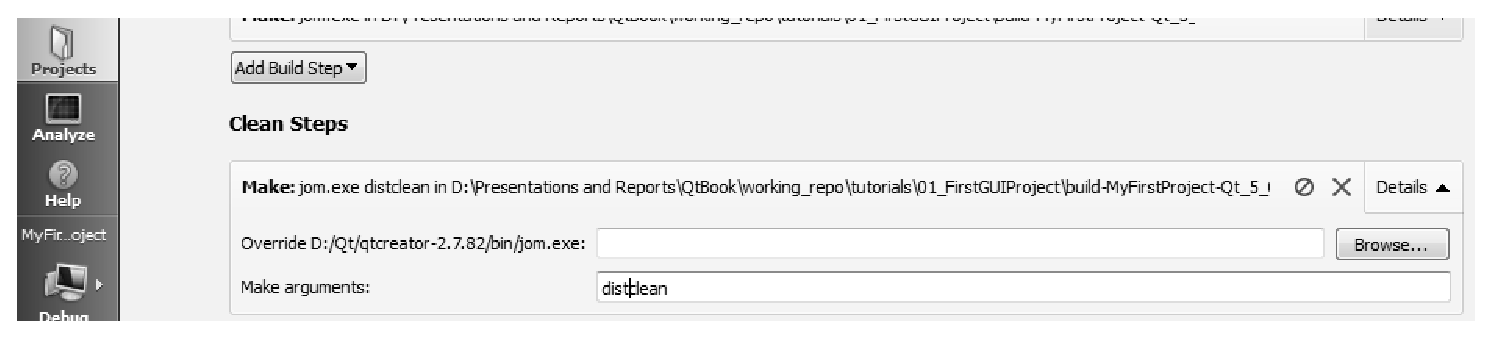
\includegraphics[width=0.7\textwidth]{img/ris_12_2}
\caption{Настройки очистки проекта}
\label{ch12:refDrawing1}
\end{center}
\end{figure}

Снова очистите проект --- все сгенерованные файлы, включительно с исполняемым файлом и \Sys{make}-файлами, будут
удалены.

\section[Консольный проект \Sys{Qt}.Вывод сообщений.]{Консольный проект \Sys{Qt}. Вывод сообщений.}
\index{Консольный проект}Несмотря на то, что \Sys{Qt} почти всегда рассматривают как
инструментарий для создания программ с графическим интерфейсом, его также можно использовать и в таких программах,
которые работают как фоновые процессы, а также в консольных проектах. Для нескольких следующих примеров
мы будем использовать последний созданный нами в предыдущем разделе проект.

В таком консольном проекте можно использовать почти все привычные для \Sys{Qt} средства и классы. В следующих
нескольких примерах мы рассмотрим работу с некоторыми важными типами \Sys{Qt} именно на примере
консольного проекта. А пока что ограничимся только обзором средства, которое позволяет выводить в консоль сообщения и
разнообразную информацию для отладки в процессе работы программы.

Для вывода информации в консольном  проекте можно использовать все привычные средства
стандартной библиотеки \Sys{C++}. Но в \Sys{Qt} для этого есть удобный инструмент --- функция
\index{Функция!qDebug}\Sys{qDebug()}. Рассмотрим пример её использования:
\begin{lstlisting}
#include <QDebug>
//`Собственный тип данных --- структура для комплексных чисел`
struct complex
{
    double re;
    double im;
};
//`Определение потокового оператора для поддержки вывода собственного типа`
//`complex с помощью qDebug()`
QDebug operator<<(QDebug dbg, const complex &c)
{
    dbg.nospace() << "(" << c.re << " + i*" << c.im << ")";
    return dbg.space();
}
int main(int lArgc, char *lArgv[])
{
    //`Вывод разнообразных типов данных`
    qDebug() << "Hello, " << "this is debug output";
    qDebug() << "Integer values: " << 1 << 10 << 100;
    qDebug() <<"Doubles and floats: "<<.1 << .123 << 0.112345;
    qDebug() << "Characters: " << 'c' << '\t' << '$' << '\n' << "newline";
    qDebug() << "Booleans: " << true << false;
    qDebug() << "Pointers: " << lArgv;
    qDebug() << " and much more...";
    //`Вывод собственного типа данных`
    complex c;
    c.re = 0.2;
    c.im = 1.5;
    qDebug() << "including custom types: " << c;
    return 0;
}
\end{lstlisting}

После выполнения программы в консоли увидим текст:
\begin{verbatim}
Hello, this is debug output 
Integer values: 1 10 100 
Doubles and floats: 0.1 0.123 0.112345 
Characters: c    $ 
newline 
Booleans: true false 
Pointers: 0x3278fc8 
and much more... 
including custom types: (0.2 + i*1.5)
\end{verbatim} 

Кроме \Sys{qDebug()} существуют другие функции для вывода сообщений разного уровня.
Описание и примеры этих функций рассмотрим в таблице~\ref{ch12:refTable1}.

{\noindent\small\tabcolsep=0.3em
\begin{longtable}{|p{0.135\textwidth}|p{0.18\textwidth}|p{0.28\textwidth}|p{0.33\textwidth}|}
\caption{Функции для вывода сообщений} \label{ch12:refTable1}\\
\hline
\Emph{Функция}&\Emph{Описание}&\Emph{Особенности}&\Emph{Пример}\\
\hline \hline
\endfirsthead
\multicolumn{4}{c}%
{{\tablename\ \thetable{} --- продолжение}} \\
\hline
\Emph{Функция}&\Emph{Описание}&\Emph{Особенности}&\Emph{Пример}\\
\hline \hline
\endhead
\index{Функция!qDebug}\Sys{qDebug()} &
Вывод сообщений для отладки, разнообразной информации при работе программы. &
Сообщения могут быть выключены с помощью специального макроопределения
{\scriptsize\index{Макрос!QT\_NO\_DEBUG\_OUTPUT}\Sys{QT\_NO\_DEBUG\_OUTPUT}} 
например, в файле проекта:
\begin{lstlisting}
DEFINES += 
  QT_NO_DEBUG_OUTPUT 
\end{lstlisting}
&
\begin{lstlisting}
int error_num = 59;
std::string error_string("uknown error");
qDebug("result: %d, description: %s", error_num, error_string.c_str());
------------------
#include <QDebug>
...
qDebug()<<"result: " <<error_num <<", description:" <<error_string.c_str();
\end{lstlisting}
\\\hline
\index{Функция!qWarning}\Sys{qWarning()} &
Вывод сообщений при  работе программы. &
Сообщения могут быть выключены с помощью специального макроопределения
{\scriptsize\index{Макрос!QT\_NO\_WARNING\_OUTPUT}\Sys{QT\_NO\_WARNING\_OUTPUT}} 
например, в файле проекта:
\begin{lstlisting}
DEFINES += 
  QT_NO_WARNING_OUTPUT
\end{lstlisting}
&
\begin{lstlisting}
qWarning("warning: %d, description: %s", error_num, error_string.c_str());
------------------
#include <QDebug>
...
qWarning()<<"warning: " <<error_num <<", description:" <<error_string.c_str();
\end{lstlisting}
\\\hline
\index{Функция!qCritical}\Sys{qCritical()} &
Вывод сообщений о критических  ошибках. &
 &
\begin{lstlisting}
qCritical("critical error: %d, description:%s",error_num, error_string.c_str());
------------------
#include <QDebug>
...
qCritical()<<"critical error: " <<error_num  <<", description:" <<error_string.c_str();
\end{lstlisting}
\\\hline
\index{Функция!qFatal}\Sys{qFatal()} &
Вывод сообщений о фатальных для программы ошибках. &
После вывода сообщения  происходит аварийное завершение работы программы. &
\begin{lstlisting}
qFatal("fatal error: %d, description:%s", error_num, error_string.c_str());
\end{lstlisting}
\\\hline
\end{longtable}
}

\section[Работа с текстовыми строками в Qt]{Работа с текстовыми строками в Qt. Класс QString. Списки строк QStringList.}

Обычные строки С довольно просты в использовании, но работать с ними не очень удобно в ряде
случаев. Один из них, это поддержка выбора кодировок для
текста. Ведь, как известно, существует много разных стандартов кодирования символов текста, которые
отличаются поддержкой разного диапазона кодируемых символов.

В \Sys{Qt} для работы со строками есть мощный и  специализированный класс ---
\index{Класс!QString}\Sys{QString}. Он имеет поддержку Unicode, возможность преобразования
текста между разными кодировками и в обычные строки \Sys{С} и \Sys{std::string}. А также он имеет хорошее быстродействие и богатый
набор инструментов для работы. Поддержка Unicode позволяет работать с текстом на любом языке мира, что очень важно при
локализации графического интерфейса программы.

Рассмотрим методы работы с текстовыми строками в \Sys{Qt}. Перед началом работы с текстом в \Sys{Qt} нужно подключить
файл описания \Sys{QString}:\\
\lstinline!#include <QString>!

Как и почти для всех классов \Sys{Qt}, \emph{название класса совпадает с названием файла
описания класса}, который необходимо подключить с помощью директивы \Sys{\#include}.

Существует большое количество разных способов добавления строк и символов к существующей строке:
\begin{lstlisting}
QString lMainStr = "string"; //lMainStr == "string"
lMainStr += ' '; //lMainStr == "string "
(lMainStr += "is") += ' '; //lMainStr == "string is"
QString lHelperStr1("composed");
lMainStr += lHelperStr1; // lMainStr == "string is composed"
QString lHelperStr2 = + ' ' +QString("from") + ' ';
lMainStr.append(lHelperStr2);
// lMainStr == "string is composited from "
lMainStr.push_back("fragments");
// lMainStr == "string is composited from fragments"
lMainStr.prepend("This ");
//lMainStr == "This string is composited from fragments"
lMainStr.insert(lMainStr.length(), ".");
//lMainStr == "This string is composited from fragments."
lMainStr += QString(2, '.');
//lMainStr == "This string is composited from fragments..."
lMainStr= lMainStr.rightJustified(lMainStr.length() + 8, ' ');
//lMainStr=="This string is composited from fragments..."
\end{lstlisting}

Также есть возможность выделения части строки либо разделения её на части:
\begin{lstlisting}
QString lQuote= "This is sentence one. This is sentence two.";
//`Новая строка с пяти символов`
QString lFragment1 = lQuote.left(5); // lFragment1 == "This "
qDebug() << "lFragment1 is: " << lFragment1;
//`Первое предложение: Все символы до первой точки`
QString lSentence = lQuote.section('.', 0, 0);
qDebug() << "lSentence is: " << lSentence;
// lSentence == "This is sentence one"
//`Cписок слов в строке`
QStringList lWordsList = lSentence.split(' ', QString::SkipEmptyParts);
qDebug() << lWordsList;
// lWordsList == ("This", "is", "sentence", "one", "This",
// "is", "sentence", "two")
\end{lstlisting}

Для проверки на пустую строку используют метод \Sys{isEmpty()}. Его не следует путать с
методом \Sys{isNull()}, который возвращает значение \Sys{true} только для ещё не
инициализированной строки. Например:
\begin{lstlisting}
QString().isNull();       //true (`нулевая строка`)
QString().isEmpty();      //true (`нулевая строка тоже пустая`)
Qstring("").isNull();     //false (`пустая строка не является нулевой`)
QString("").isEmpty();    // true
QString("abc").isNull();  // false
QString("abc").isEmpty(); // false
\end{lstlisting}

\Sys{QString} имеет инструменты для преобразования из \Sys{std::string} и наоборот.
Например:
\begin{lstlisting}
QString lQtStringInitial = "I am a standard STL string.";
std::string lStdString = lQtStringInitial.toStdString();
QString lQtString = QString::fromStdString(lStdString);
\end{lstlisting}

Также \Sys{QString} имеет  средства для работы с числовой информацией:
\begin{lstlisting}
//`преобразование целого числа в строку`
int x = 16;
QString lXStr = QString::number(x);
// x = 7; lXStr  = 7
//`преобразование строки в целое число`
int y = lXStr.toInt();
//`преобразование дробного числа в строку`
double teta = 12099.10012021210102109991;
QString lTetaStr = QString::number(teta);
// lTetaStr == 12099.1
lTetaStr.setNum(teta);
// lTetaStr == 12099.1
//`вывод с 4-мя знаками после запятой`
lTetaStr = QString::number(teta,'f',4);
// lTetaStr == 12099.1001
//`форматирование с использованием символа 'e'`
lTetaStr = QString::number(teta,'e');
// lTetaStr == 1.209910e+04
//`Запись числа в строку в разных системах счисления`
lXStr = QString(int %1 is %L2 in decimal system, %L3 in binary system, and %L4 in hexadecimal)
    .arg(x)
    .arg(x, 0, 10)
    .arg(x, 0, 2)
    .arg(x, 0, 16);
\end{lstlisting}

Для работы со списком строк в \Sys{Qt} предусмотрен специализированный тип
\index{Класс!QStringList}\Sys{QStringList}.  \Sys{QStringList} относят к контейнерным классам \Sys{Qt}.
Подробнее классы-контейнеры мы рассмотрим в следующем параграфе.

\section[Контейнерные классы в \Sys{Qt}]{Контейнерные классы в \Sys{Qt}}

Список строк \Sys{QStringList}, который мы рассматривали, является представителем
семейства \index{Контейнерные классы \Sys{Qt}}контейнерных классов \Sys{Qt}, которые являются
аналогом контейнеров \Sys{STL}. Но в то же время они имеют свои собственные различия в 
реализации и возможностях. Мы же будем
в дальнейшем использовать в наших примерах исключительно контейнеры \Sys{Qt}.

Простейшим контейнерным классом является \Sys{QList}. \index{Класс!QList}\Sys{QList}
 --- список общего назначения. Для добавления элементов в начало и в конец списка используют методы
\Sys{prepend()} и \Sys{append()}. Также можно добавить несколько элементов за раз
используя потоковые операторы. Например:
\begin{lstlisting}
#include <QList>
    ...
QList<QString> lList;
QString lStr1("string1");
QString lStr2("string2");
lList << lStr1 << lStr2; //`Добавляем несколько элементов за раз`
lList.prepend(lStr1); //`Добавляем элемент в начало (повторно)` 
lList.append("string3"); //`Добавляем в конец списка`
lList << "string4";	//`То же, что и` lList.append("string4");
\end{lstlisting}

Последние две строки возможны за счёт неявного преобразования \Sys{char*} в
\Sys{QString}. Класс \Sys{QStringList}, которого мы коснулись в примерах
предыдущего раздела посвящённого текстовым строкам, наследует от \Sys{QList{<}QString{>}}
и реализует ряд дополнительных методов для работы со строками в списке.

Для доступа к элементам используют метод \Sys{at()}, который принимает индекс элемента в
списке в качестве аргумента. Количество элементов в списке возвращают методы \Sys{size()} и
\Sys{count()}.
\begin{lstlisting}
qDebug() << lList.first();
qDebug() << lList.last();
if(lList.size()>3) qDebug() << lList.at(3);
\end{lstlisting}

Также стоит отметить два других важных разновидности контейнеров: хэш
(\index{Класс!QHash}\Sys{QHash}) и словарь
(\index{Класс!QMap}\Sys{QMap}). Хэш --- контейнер, в котором элементы добавляют парами
(ключ-значение). Значение в хэше находят по
ключу, а для поиска используют хэш-функцию, которая преобразует ключ
в значение. В словаре элементы также добавляют парами ключ-значение, но значение
сортируют по ключу. Для доступа к значению, используют метод \Sys{value()}, который принимает два
параметра: ключ и значение по умолчанию, которое метод вернёт, если значение не будет
найдено. Например:
\begin{lstlisting}
#include <QMap>
    ...
QMap<QString, QString> lSurnameByName;
lSurnameByName.insert("Bill", "Hunter");
lSurnameByName.insert("Marry", "Lee");
//`Поиск значения по ключу`
qDebug() << "Bill" << lSurnameByName.value("Bill");
qDebug() << "Marry" << lSurnameByName.value("Marry", "Doe");
//`Прибавляем другое значение с уже существующим ключом`
lSurnameByName.insert("Marry", "Hunter");
qDebug() << "Marry" << lSurnameByName.value("Marry");
//`Ключи не существуют --- вывод значений по умолчанию`
qDebug() << "James" << lSurnameByName.value("James");
qDebug() << "John" << lSurnameByName.value("John", "Doe");
\end{lstlisting}

После выполнения получим вывод:
\begin{verbatim}
Bill "Hunter" 
Marry "Lee" 
Marry "Hunter" 
James "" 
John "Doe"
\end{verbatim}

Обратите внимание: после того, как мы добавили ещё одно значение с тем же ключом (Marry),
предыдущее значение было перезаписано новым
значением. Для того, чтобы добавить несколько значений с одним и тем же ключом можно
воспользоваться методом \Sys{insertMulti()}.
\begin{lstlisting}
#include <QHash>
    ...
QHash<QString, QString> lClassificationHash;
//`Добавляем несколько значений с одинаковыми ключами`
lClassificationHash.insertMulti("fruits", "apple");
lClassificationHash.insertMulti("fruits", "orange");
lClassificationHash.insertMulti("vegetables", "potato");
lClassificationHash.insertMulti("vegetables", "cabbage");
lClassificationHash.insertMulti("vegetables", "tomato");
qDebug()<<lClassificationHash.value("fruits");//`Вывод одного значения с ключом`
qDebug()<<lClassificationHash.values("fruits"); //`Вывод значений с ключом`
qDebug()<<lClassificationHash.values("vegetables");
\end{lstlisting}

Получим следующий вывод в консоль:
\begin{verbatim}
"orange" 
("orange", "apple") 
("tomato", "cabbage", "potato")
\end{verbatim}

Для итерации по списку можно воспользоваться макросом
\index{Макрос!foreach}\Sys{foreach}. Также можно
воспользоваться итератором в стиле Java. Например:
\begin{lstlisting}
QList<int> lList; //`Создаём список целых чисел`
lList.append(3);  //`Добавляем элементы`
lList.append(6);
lList.append(9);
QListIterator<int> lIt(lList); //`Создаём итератор для списка`
while (lIt.hasNext()) //`Пока следующий элемент существует`
{
  qDebug() << lIt.next(); //`...вывести следующий элемент`
}
\end{lstlisting}

Другой пример --- итерация в обратном направлении. На этот раз используем хеш.
\begin{lstlisting}
QHash<QString, int> lNumberByName;
lNumberByName.insert("twelve", 12);
lNumberByName.insert("thirty three", 33);
lNumberByName.insert("one hundred an twenty five", 125);
QHashIterator<QString, int> lHashIterator(lNumberByName);
lHashIterator.toBack(); //`Перейти к концу контейнера --- итератор указывает после` 
                        //`последнего элемента`
while (lHashIterator.hasPrevious())
{
  lHashIterator.previous();//`Переходим к предыдущемму элементу`
  //`Выводим ключ и значение`
  qDebug() << lHashIterator.key()<< " - " << lHashIterator.value();
}
\end{lstlisting}

Следующий пример  --- с итератором в стиле \Sys{STL}.
\begin{lstlisting}
QHash<QString, int>::const_iterator lStlLikeIterator;
for (lStlLikeIterator = lNumberByName.begin();
    lStlLikeIterator != lNumberByName.end();
    lStlLikeIterator++)
    {
      qDebug() << lStlLikeIterator.key()<< " - "
      //`Тоже самое, что и` *lStlLikeIterator
      << lStlLikeIterator.value();
    }
\end{lstlisting}

В таблице~\ref{ch12:refTable2} приведены разновидности контейнеров~\Sys{Qt}. 

{\noindent\small
\begin{longtable}{|p{0.18\textwidth}|p{0.74\textwidth}|}
\caption{Контейнеры \Sys{Qt}} \label{ch12:refTable2}\\
\hline
\Emph{Переменная}&\Emph{Описание особенностей}\\
\hline \hline
\endfirsthead
\multicolumn{2}{c}%
{{\tablename\ \thetable{} --- продолжение}} \\
\hline
\Emph{Переменная}&\Emph{Описание особенностей}\\
\hline \hline
\endhead
\index{Класс!QList}\Sys{QList} & Список общего назначения для использования в большинстве ситуаций, которые возникают при 
разработке. Имеет оптимальное быстродействие в большинстве случаев.\\\hline
\index{Класс!QLinkedList}\Sys{QLinkedList} & Реализует связный список в \Sys{Qt}. Отсутствует операция доступа по индексу элемента (такая как \Sys{at(int pos)}). \\\hline
\index{Класс!QVector}\Sys{QVector} &Реализует вектор элементов в \Sys{Qt}.\\\hline
\index{Класс!QStack}\Sys{QStack} &Реализует стек. Стек размещает элементы по принципу LIFO (Last In, First Out) --- элемент, добавленный первым будет последним элементом в стеке.\\\hline
\index{Класс!QQueue}\Sys{QQueue} &Реализует очередь. Очередь размещает элементы по принципу FIFO (First In, First Out) --- элемент, добавленный первым, будет первым элементом в очереди.\\\hline
\index{Класс!QSet}\Sys{QSet} & Множество элементов. Гарантирует, что все элементы будут  уникальными.\\\hline
\index{Класс!QMap}\Sys{QMap} &Контейнерный класс для словаря. Элементы добавляют парами: ключ-значение. Словарь всегда сортирует элементы по ключу. Позволяет найти элемент по ключу.\\\hline
\index{Класс!QMultiMap}\Sys{QMultiMap} & Контейнерный класс словаря создан для удобной работы с тем, чтобы каждому ключу соответствовало несколько значений. Метод insert() не заменяет значение ключа, если ключ уже существует, а добавляет новую пару ключ-значение.\\\hline
\index{Класс!QHash}\Sys{QHash} & Контейнерный класс для хеша. Элементы добавляют парами: ключ --- значение. Элементы хранятся в хеше в произвольном порядке. Позволяет выполнять очень быстрый поиск  элемента по ключу.\\\hline
\index{Класс!QMultiHash}\Sys{QMultiHash} & Контейнерный класс хеша, создан для удобной работы с тем, чтобы каждому ключу соответствовало несколько значений. Метод \Sys{insert()} не заменяет значение ключа, если ключ уже
существует, а добавляет новую пару ключ-значение.\\\hline
\end{longtable}
}

\section[Работа с файлами]{Работа с файлами}
Инструментарий \Sys{Qt} содержит большое количество средств, которые позволяют разработчику абстрагироваться от
деталей реализации на той или иной программной платформе. В этом разделе мы рассмотрим средства, \Sys{Qt} предоставляет для
работы с файловой системой.

Все устройства ввода/вывода в \Sys{Qt} наследуют от абстрактного класса
\index{Класс!QIODevice}\Sys{QIODevice}. Среди его потомков: буфер для данных
(\Sys{QBuffer}), процесс --- программа которая выполняется в системе (\Sys{QProcess}),
сетевой сокет (\Sys{QAbstractSocket}) и другие. Мы же подробно рассмотрим работу с
другим его потомком --- классом для работы с файлом (\index{Класс!QFile}\Sys{QFile}).

Для работы с файлом необходимо создать объект класса \Sys{QFile} и задать для него
путь к файлу (абсолютный или относительный), с которым вы будете работать. Путь и имя передают как параметр
конструктора или с помощью метода \Sys{setFileName()}.

Далее файл необходимо открыть и задать режим доступа к нему. Метод \Sys{open()}
принимает флаги доступа и возвращает \Sys{true}, если
файл удалось открыть. Доступные флаги доступа:
\begin{itemize}
\item \Sys{QIODevice::ReadOnly} --- открыть для чтения;
\item \Sys{QIODevice::WriteOnly} --- открыть для записи;
\item \Sys{QIODevice::ReadWrite} --- открыть для чтения и записи;
\item \Sys{QIODevice::Append} --- все данные будут добавляться в конец файла (после уже существующих
данных);
\item \Sys{QIODevice::Truncate} --- если возможно, стереть содержимое файла перед открытием;
\item \Sys{QIODevice::Text} --- режим работы с текстовым файлом (важно для
текстовых файлов для корректной обработки символов завершения строки в \Sys{Windows} и \Sys{Linux}).
\end{itemize}

Флаги (класс \index{Класс!QFlags}\Sys{QFlags}) часто используют в \Sys{Qt} для
задания комбинации настроек. Для комбинации нескольких настроек, так же как и бинарной арифметике, используют операцию
побитового \Sys{OR}.

\index{Чтение файла с использованием \Sys{Qt}}Для записи и чтения используют методы
\Sys{read()} и \Sys{write()}, которые перегружены в нескольких вариантах. Для
чтения одной строки текстового файла используют метод \Sys{readLine()}.
Для чтения всего содержимого можно воспользоваться методом \Sys{readAll()}. Текущую
позицию при чтении из файла определяют с помощью метода \Sys{pos()}. Установить позицию можно с
помощью метода \Sys{seek()}. Метод \Sys{atEnd()} позволяет определить достигли ли
мы конца файла при чтении. После завершения работы с файлом его нужно закрыть вызовом метода \Sys{close()}.
Следующий пример демонстрирует чтение текстового файла и вывод его в консоль.
\begin{lstlisting}
#include <QDebug>
#include <QFile>
int main(int argc, char *argv[])
{
  const QString lFileName("file.txt");
  //`Проверяем существование файла`
  if (!QFile::exists(lFileName))
  {
    qCritical("File %s does not exists.",
    qPrintable(lFileName));
    return 1;
  }
  QFile lFile;
  //`Устанавливаем имя файла`
  lFile.setFileName(lFileName);
  //`Открываем файл --- текстовый, только для чтения`
  if (!lFile.open(QIODevice::ReadOnly|QIODevice::Text))
  {
  //`Если открыть файл не удалось --- выводим сообщение об ошибке`
    qCritical("Error %d : %s.", lFile.error(),
    qPrintable(lFile.errorString()));
    return 2;
  }
  //`Пока можно прочесть строку`
  while (!lFile.atEnd())
  {
    // `... выводить её в консоль`
    qDebug() << lFile.readLine();
  }
  //`Заканчиваем работу с файлом`
  lFile.close();
  return 0;
}
\end{lstlisting}

\index{Запись файла с использованием \Sys{Qt}}Рассмотрим работу с файлами в \Sys{Qt} на другом примере
записи и чтения текстовой информации. В этом примере мы используем класс
\index{Класс!QTextStream}\Sys{QTextStream} для получения введённой пользователем
информации в стандартный поток ввода. Конструктор \Sys{QTextStream} может принимать в качестве
параметра указатель на потомок \Sys{QIODevicе}, указатель на \Sys{QString}
или \Sys{QByteArray}, а также файловую переменную. В примере мы перенаправляем
поток ввода в \Sys{QТextStream}. Далее мы читаем строку
из потока ввода и записываем её в файл.
\begin{lstlisting}
#include <QDebug>
#include <QIODevice>
#include <QFile>
#include <QTextStream>
int main(int lArgc, char *lArgv[])
{
  QTextStream in(stdin);
  QFile lFile("in.txt");
  if (lFile.open(QIODevice::WriteOnly | QIODevice::Truncate))
  {
    QString lData = in.readLine();
    lFile.write(qPrintable(lData));
    lFile.close();
  }
  else
  {
    qDebug() << "Cannot open file!";
  }
  return 0;
}
\end{lstlisting}

В следующем фрагменте демонстрируем обратный процесс --- чтение строки из файла и вывод прочитанного строки
в консоль. \index{Чтение файла с использованием \Sys{Qt}}Опять же для чтения из файла мы
используем \Sys{QTextStream}.
\begin{lstlisting}
QFile lFile("in.txt");
if (lFile.open(QIODevice::ReadOnly | QIODevice::Truncate))
{
  QTextStream in(&lFile);
  QString lData = in.readLine();
  qDebug() << lData;
  lFile.close();
}
else
{
  qDebug() << "Cannot open file!";
}
\end{lstlisting}


\section{Задачи для самостоятельного решения}
\begin{enumerate}
\item Создайте пустой консольный проект \Sys{Qt} и скомпилируйте его. Определите потоковый оператор для вывода
класса Person, который имеет поля Name, Phone number, Address для вывода в консоль с помощью функции qDebug(). 
\item Создайте программу табуляции функции и записи в текстовый файл с использованием средств,
предоставляемых \Sys{Qt}. Используйте классы QFile, QTextStream для записи. Адрес текстового файла жёстко задайте в тексте
программы. 
\item Создайте программу чтения значений протабулированной функции из
текстового файла с использованием средств \Sys{Qt} и вывода значений в консоль. Используйте классы QFile, QTextStream для
чтения. Адрес текстового файла жёстко задайте в тексте программы. Если файл невозможно открыть для чтения --- выведите
сообщение о критической ошибке с завершением работы программы. 
\end{enumerate}
